\documentclass[border=2pt]{standalone}
\usepackage{pgfplots}
\usepgfplotslibrary{statistics}
\pgfplotsset{compat=1.18}
\begin{document}
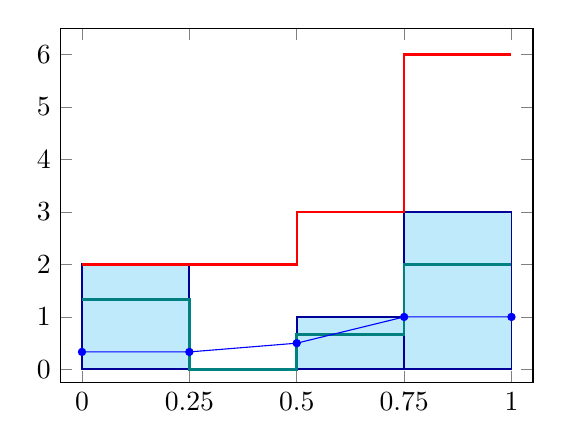
\begin{tikzpicture}
\begin{axis}[
    width=60mm,height=45mm,scale only axis,
    xmin=-0.05,xmax=1.05,ymin=-0.25,ymax=6.5,
    xtick={0,0.25,0.5,0.75,1},ytick={0,1,2,3,4,5,6},
    hist/data=x,hist/bins=4,hist/data min=0,hist/data max=1,
]
    \addplot[draw=blue!60!black,fill=cyan!25,line width=0.7pt,hist]
        coordinates {(0.75,1.5) (0,4) (1,3.5) (0.5,1.5) (0.125,2.7) (0.875,0.25)};
    \addplot[teal,no marks,line width=1pt,hist={density,handler/.style={const plot}}]
        coordinates {(0.75,1.5) (0,4) (1,3.5) (0.5,1.5) (0.125,2.7) (0.875,0.25)};
    \addplot[red,no marks,line width=0.8pt,hist={cumulative,handler/.style={const plot}}]
        coordinates {(0.75,1.5) (0,4) (1,3.5) (0.5,1.5) (0.125,2.7) (0.875,0.25)};
    \addplot[blue,mark=*,mark size=1.3pt,hist={cumulative,density,handler/.style={sharp plot}}]
        coordinates {(0.75,1.5) (0,4) (1,3.5) (0.5,1.5) (0.125,2.7) (0.875,0.25)};
\end{axis}
\end{tikzpicture}
\end{document}
